% ------------------------------------------------------------------------------
% TYPO3 CMS 8.4 - What's New - Chapter "Deprecated Functions" (German Version)
%
% @author	Michael Schams and Patrick Lobacher
% @license	Creative Commons BY-NC-SA 3.0
% @link		http://typo3.org/download/release-notes/whats-new/
% @language	German
% ------------------------------------------------------------------------------
% LTXE-CHAPTER-UID:		3f842373-9262b8d3-f9c8de76-cf29ce17
% LTXE-CHAPTER-NAME:	Deprecated Functions
% ------------------------------------------------------------------------------

\section{Veraltete/Entfernte Funktionen}
\begin{frame}[fragile]
	\frametitle{Veraltete/Entfernte Funktionen}

	\begin{center}\huge{Kapitel 5:}\end{center}
	\begin{center}\huge{\color{typo3darkgrey}\textbf{Veraltete/Entfernte Funktionen}}\end{center}

\end{frame}

% ------------------------------------------------------------------------------
% LTXE-SLIDE-START
% LTXE-SLIDE-UID:		0c17ce7d-d853a76f-36e902e1-65b3eef8
% LTXE-SLIDE-ORIGIN:	cf7400eb-0f683329-f6c51cbf-dfd192d9 English
% LTXE-SLIDE-TITLE:		#77630: Remove wizard icons
% ------------------------------------------------------------------------------
\begin{frame}[fragile]
	\frametitle{Veraltete/Entfernte Funktionen}
	\framesubtitle{Wizard Icons entfernt}

	\begin{itemize}

		\item Die folgenden Icons wurden vom \texttt{FormFieldWizard} entfernt:

			\begin{itemize}
				\item \texttt{wizard\_add.gif}
				\item \texttt{wizard\_edit.gif}
				\item \texttt{wizard\_link.gif}
				\item \texttt{wizard\_list.gif}
				\item \texttt{wizard\_rte.gif}
				\item \texttt{wizard\_table.gif}
			\end{itemize}

	\end{itemize}

	\begin{figure}
		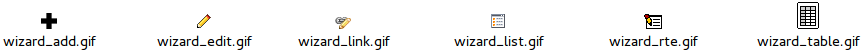
\includegraphics[width=0.95\linewidth]{DeprecatedRemovedFunctions/77630.png}
	\end{figure}

\end{frame}

% ------------------------------------------------------------------------------
% LTXE-SLIDE-START
% LTXE-SLIDE-UID:		fe319bb8-25de2a65-7629ef35-a9eb6887
% LTXE-SLIDE-ORIGIN:	d5ced5e7-04dffe16-b8ec9f2c-712020cd English
% LTXE-SLIDE-TITLE:		#77693: Remove/Move Icons from EXT:t3skin
% ------------------------------------------------------------------------------

\begin{frame}[fragile]
	\frametitle{Veraltete/Entfernte Funktionen}
	\framesubtitle{Icons von \texttt{EXT:t3skin}}

	\begin{itemize}

		\item Die folgenden Icons von \texttt{EXT:t3skin} wurden entfernt oder verschoben
		\item \textbf{Entfernt:}

			\begin{itemize}
				\item \smaller\texttt{typo3/sysext/t3skin/icons/gfx/error.png}
				\item \texttt{typo3/sysext/t3skin/icons/gfx/i/\_icon\_ftp.gif}
				\item \texttt{typo3/sysext/t3skin/icons/gfx/information.png}
				\item \texttt{typo3/sysext/t3skin/icons/gfx/notice.png}
				\item \texttt{typo3/sysext/t3skin/icons/gfx/warning.png}
			\end{itemize}

		\item \textbf{Verschoben:}

			\begin{itemize}
				\item \smaller\texttt{typo3/sysext/t3skin/icons/gfx/icon\_fatalerror.gif}
				\item \texttt{typo3/sysext/t3skin/images/icons/status/status-edit-read-only.png}
				\item \texttt{typo3/sysext/t3skin/images/icons/status/warning-in-use.png}
				\item \texttt{typo3/sysext/t3skin/images/icons/status/warning-lock.png}
				\item \texttt{typo3/sysext/t3skin/images/icons/status/status-reference-hard.png}
				\item \texttt{typo3/sysext/t3skin/images/icons/status/status-reference-soft.png}
			\end{itemize}

	\end{itemize}

\end{frame}

% ------------------------------------------------------------------------------
% LTXE-SLIDE-START
% LTXE-SLIDE-UID:		51721acd-731a3920-1ea8db59-40bb91f5
% LTXE-SLIDE-ORIGIN:	7848f0b0-d687b337-f7638646-680dc819 English
% LTXE-SLIDE-TITLE:		Obsolete page tree and click menu settings removed
% ------------------------------------------------------------------------------

\begin{frame}[fragile]
	\frametitle{Veraltete/Entfernte Funktionen}
	\framesubtitle{Seitenbaum- und Click-Menu-Einstellungen}

	\begin{itemize}

		\item Die obsoleten Seitenbaum- und Click-Menu-Einstellungen wurden entfernt
		\item \textbf{Eigenschaften}:

		\begin{itemize}
			\item \texttt{FileSystemNavigationFrameController->doHighlight}
			\item \texttt{ClickMenu->leftIcons}
		\end{itemize}

		\item \textbf{TypoScript-Einstellungen}:

		\begin{itemize}
			\item \texttt{options.pageTree.disableTitleHighlight}
			\item \texttt{options.contextMenu.options.leftIcons}
		\end{itemize}

	\end{itemize}

\end{frame}

% ------------------------------------------------------------------------------
% LTXE-SLIDE-START
% LTXE-SLIDE-UID:		178d3d26-1c587d89-e54a82bc-40207987
% LTXE-SLIDE-ORIGIN:	aad23a73-7b046eaf-fb4bb862-2f88ef71 English
% LTXE-SLIDE-TITLE:		ExtensionManagementUtility::extRelPath()
% LTXE-SLIDE-REFERENCE:	#78193: ExtensionManagementUtility::extRelPath() deprecated
% ------------------------------------------------------------------------------

\begin{frame}[fragile]
	\frametitle{Veraltete/Entfernte Funktionen}
	\framesubtitle{ExtensionManagementUtility::extRelPath()}

	\begin{itemize}

		\item Die Methode \texttt{ExtensionManagementUtility::extRelPath()} wurde als veraltet markiert\newline
			\small(diese wurde benutzt, um relative Pfade zum aktuellen Script aufzulösen)\normalsize
		\item Alternativ kann folgendes verwendet werden:

			\begin{itemize}
				\item \texttt{ExtensionManagementUtility::extPath()}\newline
					\smaller(um den vollen Pfad zu einer Extension zu ermitteln)\normalsize
				\item \texttt{ExtensionManagementUtility::siteRelPath()}\newline
					\smaller(um die Location einer Extension relativ zu \texttt{PATH\_site} zu ermitteln\normalsize
				\item \texttt{GeneralUtility::getFileAbsFileName()}\newline
					\smaller(um eine Datei/einen Pfad mit dem Prefix \texttt{EXT:myextension} zu ermitteln)\normalsize
				\item \texttt{PathUtility::getAbsoluteWebPath()}\newline
					\smaller(um die Location einer Datei auszugeben, die absolut referenziert wurde)\normalsize
			\end{itemize}

	\end{itemize}

\end{frame}

% ------------------------------------------------------------------------------
% LTXE-SLIDE-START
% LTXE-SLIDE-UID:		a8589498-fe4274e2-5b24cfe1-970706b6
% LTXE-SLIDE-ORIGIN:	43a5eaf5-8945a8d5-ac27d4ea-24ffc8e3 English
% LTXE-SLIDE-TITLE:		Miscellaneous (1) (#75363)
% LTXE-SLIDE-REFERENCE:	#75363: Deprecate FormResultCompiler->JStop()
% LTXE-SLIDE-REFERENCE:	#75637: Deprecate optional parameters of RecyclerUtility::getRecordPath()
% ------------------------------------------------------------------------------

\begin{frame}[fragile]
	\frametitle{Veraltete/Entfernte Funktionen}
	\framesubtitle{Miscellaneous (1)}

	\begin{itemize}
		\item Die Methode \texttt{FormResultCompiler->JStop()} wurde in \texttt{addCssFiles()} umbenannt.
			Der alte Methoden-Namen ist als veralteter Alias erhalten geblieben und wird mit TYPO3 v9 entfernt.

		\item Die Methode \texttt{ClickMenu::DB\_editPageProperties()} wurde als veraltet deklariert.

		\item Die folgenden Argumente der Methode \texttt{RecyclerUtility::getRecordPath()} wurden als veraltet deklariert:

			\begin{itemize}
				\item \texttt{\$clause}
				\item \texttt{\$titleLimit}
				\item \texttt{\$fullTitleLimit}
			\end{itemize}

	\end{itemize}

\end{frame}

% ------------------------------------------------------------------------------
% LTXE-SLIDE-START
% LTXE-SLIDE-UID:		3d094f9d-a97ee100-1518baf6-69046a21
% LTXE-SLIDE-ORIGIN:	0745e3f3-83db03d7-ac24e92a-300391ba English
% LTXE-SLIDE-TITLE:		Miscellaneous (2) (#77783 and #77826)
% LTXE-SLIDE-REFERENCE:	#77783: Unused ExtJS JavaScript libraries removed
% LTXE-SLIDE-REFERENCE:	#77826: RTEHtmlArea Spellchecker eID removed
% ------------------------------------------------------------------------------

\begin{frame}[fragile]
	\frametitle{Veraltete/Entfernte Funktionen}
	\framesubtitle{Miscellaneous (2)}

	\begin{itemize}

		\item Die folgenden - nicht benutzten - ExtJS JavaScript Bibliotheken wurden entfernt:

			\begin{itemize}
				\item \texttt{app.SearchField}
				\item \texttt{grid.RowExpander}
				\item \texttt{ux.FitToParent}
			\end{itemize}

		\item Die RTEHtmlArea eID (\texttt{rtehtmlarea\_spellchecker}) für das dynamische Spellchecking wurde entfernt und der Entry-Point für HTTP-Requests
			\texttt{SpellCheckingController->main} als veraltet deklariert.

		\item Das Format \texttt{DateTime::ISO8601} ist inkompatibel mit ISO-8601,
			wurde aber aus behalten, um abwärts kompatibel zu sein.
			Stattdessen werden die Konstanten \texttt{DateTime::ATOM} oder \texttt{DATE\_ATOM} benutzt.

	\end{itemize}

\end{frame}

% ------------------------------------------------------------------------------
% LTXE-SLIDE-START
% LTXE-SLIDE-UID:		a493bc83-d8cf0b14-8e1c473b-22f57f27
% LTXE-SLIDE-ORIGIN:	0745e3f3-83db03d7-ac24e92a-300391ba English
% LTXE-SLIDE-TITLE:		Miscellaneous (3) (#77839, #78096 and #78222)
% LTXE-SLIDE-REFERENCE:	#77839: TYPO3/CMS/Core/QueryGenerator
% LTXE-SLIDE-REFERENCE:	#78096: Deprecate PageLayoutView::getResult with mysqli_result objects
% LTXE-SLIDE-REFERENCE:	#78222: Late generation of autoload information is deprecated
% ------------------------------------------------------------------------------

\begin{frame}[fragile]
	\frametitle{Veraltete/Entfernte Funktionen}
	\framesubtitle{Miscellaneous (3)}

	\begin{itemize}

		\item Das AMD-Modul \texttt{TYPO3/CMS/Core/QueryGenerator} wurde zu \texttt{EXT:lowlevel} verschoben\newline
			\small
				(und unbenannt zu \texttt{TYPO3/CMS/Lowlevel/QueryGenerator})
			\normalsize

		\item Die Methode \texttt{PageLayoutView::getResult()} wurde mit der Verwendung von \texttt{mysqli\_result} als ersten Parameter als veraltet deklartiert.

		\item Wenn sich TYPO3 im Non-Composer Modus befindet, wurden die Autoload-Informationen relativ spät im Bootstrap-Prozess gelasden. Dies ist nun veraltet.
	\end{itemize}

\end{frame}

% ------------------------------------------------------------------------------
